\documentclass[11pt,a4paper]{article}

\usepackage{../ve230}

\author{\href{liuyh615@sjtu.edu.cn}{Yihao Liu} (515370910207)}
\semester{Summer}
\year{2019}
\subtitle{Homework}
\subtitlenumber{2}
\blockinfo{}

\usetikzlibrary{positioning}

\begin{document}

\maketitle

\subsection{3-8}
\begin{center}
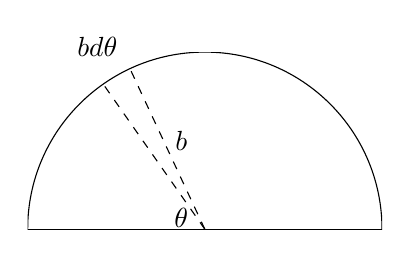
\begin{tikzpicture}[baseline=(current bounding box.north),scale=1.5]
\begin{scope}
    \clip (-1.5,0) rectangle (1.5,1.5);
    \draw (0,0) circle(1.5);
    \draw (-1.5,0) -- (1.5,0);
\end{scope}
\node[above left=0.5mm of {(115:1.5)}] {$bd\theta$};
\node at (-0.2,0.75) {$b$};
\node at (-0.2,0.1) {$\theta$};
\draw[dashed] (0,0) -- (115:1.5);
\draw[dashed] (0,0) -- (125:1.5);
\end{tikzpicture}
\end{center}

$$dQ=bd\theta\rho_l,$$
$$dE=\frac{dQ}{4\pi\epsilon_0b^2}=\frac{\rho_l}{4\pi\epsilon_0b}d\theta,$$
$$|\mathbf{E}|=\int_0^\pi dE\sin\theta=\frac{\rho_l}{4\pi\epsilon_0b}\int_0^\pi\sin\theta d\theta=\frac{\rho_l}{2\pi\varepsilon_0b}.$$
The direction is downwards.

\subsection{3-9}
\begin{center}
\begin{tikzpicture}[baseline=(current bounding box.north),scale=1.5]
\begin{scope}
    \clip (-2,-2) rectangle (2,2);
    \draw (-1.732,-1) -- (1.732,-1) -- (0,1.732) -- (-1.732,-1);
\end{scope}
\node[above left=1mm of {(-0.866,0.366)}] {$\rho_{l2}$};
\node[below=1mm of {(0,-1)}] {$-\rho_{l1}$};
\node[above right=1mm of {(0.866,0.366)}] {$\rho_{l3}$};
\end{tikzpicture}
\end{center}

$$dQ=\rho dl,$$
$$dE=\frac{dQ}{4\pi\varepsilon_0(l^2+L^2/12)}=\frac{\rho}{4\pi\varepsilon_0}\cdot\frac{dl}{l^2+L^2/12},$$
$$|\mathbf{E_1}|=\int_{-L/2}^{L/2}dE\cdot\sqrt{\frac{L^2/12}{l^2+L^2/12}}=\frac{3\rho_{l1}}{2\pi\varepsilon_0 L},$$
$$|\mathbf{E_2}|=|\mathbf{E_3}|=\frac{1}{2}|\mathbf{E_1}|=\frac{3\rho_{l1}}{4\pi\varepsilon_0 L}.$$
$$|\mathbf{E}|=|\mathbf{E_1}|-\frac{1}{2}|\mathbf{E_2}|-\frac{1}{2}|\mathbf{E_3}|=\frac{3\rho_{l1}}{4\pi\varepsilon_0 L}.$$
The direction is upwards.

\subsection{3-12}
\begin{enumerate}[label=\alph*)]
\item 
For $0<r<a$, $\mathbf{E}=\mathbf{0}$.

For $a<r<b$, $$2\pi aL\cdot\frac{\rho_{sa}}{\varepsilon_0}=2\pi rL\cdot E,$$
$$\mathbf{E}=\frac{a\rho_{sa}}{\varepsilon_0 r}\mathbf{a_r}.$$

For $b<r$, $$2\pi aL\cdot\frac{\rho_{sa}}{\varepsilon_0}+2\pi bL\cdot\frac{\rho_{sb}}{\varepsilon_0}=2\pi rL\cdot E,$$
$$\mathbf{E}=\frac{a\rho_{sa}+b\rho_{sb}}{\varepsilon_0 r}\mathbf{a_r}.$$
\item
$$\frac{a\rho_{sa}+b\rho_{sb}}{\varepsilon_0 r}=0,$$
$$a=-\frac{\rho_{sb}}{\rho_{sa}}b.$$
\end{enumerate}

\subsection{3-13}
$$W=-\int\mathbf{E}qd\mathbf{l}=2\mu \int(\mathbf{a_x}y+\mathbf{a_y}x)(\mathbf{a_x}dx+\mathbf{a_y}dy)=2\mu \int ydx+xdy.$$
\begin{enumerate}[label=\alph*)]
\item 
$$W=2\mu \int ydx+xdy=2\mu C\int_2^8 4y^2dy+2y^2dy=28\mu.$$
\item 
$$x=6y-4,$$
$$W=2\mu \int ydx+xdy=2\mu C\int_2^8 6ydy+(6y-4)dy=28\mu.$$
\end{enumerate}

\subsection{3-16}
\begin{enumerate}[label=\alph*)]
\item 
$$dQ=\rho_l dl,$$
$$dV=\frac{dQ}{4\pi\varepsilon_0\sqrt{l^2+y^2}}=\frac{\rho_l}{4\pi\varepsilon_0}\cdot\frac{dl}{\sqrt{l^2+y^2}},$$
$$V=\int_{-L/2}^{L/2}dV=\frac{\rho_l}{4\pi\varepsilon_0}\int_{-L/2}^{L/2}\frac{1}{\sqrt{l^2+y^2}} dl=\frac{\rho_l}{2\pi\varepsilon_0}{\rm arcsinh}\frac{L}{2y}.$$
\item
$$dE=\frac{dQ}{4\pi\varepsilon_0(l^2+y^2)}=\frac{\rho_l}{4\pi\varepsilon_0}\cdot\frac{dl}{l^2+y^2},$$
$$\mathbf{E}=\mathbf{a_y}\int_{-L/2}^{L/2}dE\cdot\sqrt{\frac{y^2}{l^2+y^2}}=\frac{\rho_l}{2\pi\varepsilon_0}\cdot\frac{y}{\sqrt{L^2+4y^2}}\mathbf{a_y}.$$
\item
$$-\nabla V=-\frac{dV}{dy}\mathbf{a_y}=\frac{\rho_l}{4\pi\varepsilon_0}\cdot\frac{L}{\sqrt{L^2+4y^2}}\mathbf{a_y}=\mathbf{E}.$$
\end{enumerate}

\subsection{3-19}
$$dQ=\frac{Q}{h} dz,$$
$$dV=\frac{dQ}{4\pi\varepsilon_0\sqrt{b^2+z^2}}=\frac{Q}{4\pi\varepsilon_0h\sqrt{b^2+z^2}}dz.$$
\begin{enumerate}[label=\alph*)]
\item 
$$V=\int_{z-h}^zdV=\frac{Q}{4\pi\varepsilon_0h}\int_{z-h}^z\frac{1}{\sqrt{b^2+z^2}}dz=\frac{Q}{4\pi\varepsilon_0h}\left[{\rm arcsinh}\frac{z}{b}-{\rm arcsinh}\frac{z-h}{b}\right].$$
$$\mathbf{E}=-\nabla V=-\frac{dV}{dz}\mathbf{a_z}=-\frac{Q}{4\pi\varepsilon_0h}\left[\frac{1}{\sqrt{b^2+z^2}}-\frac{1}{\sqrt{b^2+(z-h)^2}}\right]\mathbf{a_z}.$$
\item
$$V=\int_0^zdV+\int_0^{h-z}dV=\frac{Q}{4\pi\varepsilon_0h}\left[{\rm arcsinh}\frac{z}{b}+{\rm arcsinh}\frac{h-z}{b}\right].$$
$$\mathbf{E}=-\nabla V=-\frac{dV}{dz}\mathbf{a_z}=-\frac{Q}{4\pi\varepsilon_0h}\left[\frac{1}{\sqrt{b^2+z^2}}-\frac{1}{\sqrt{b^2+(h-z)^2}}\right]\mathbf{a_z}.$$
\end{enumerate}

\end{document}


